\documentclass[11pt]{article}
\usepackage[margin=1in]{geometry}
\usepackage{amsfonts, amsmath, amssymb}
\usepackage{graphicx}
\usepackage{fancyhdr}
\usepackage[nottoc, notlot, notlof]{tocbibind}
\usepackage{float}
\usepackage{caption}
\usepackage{titlesec}
\PassOptionsToPackage{hyphens}{url}\usepackage{hyperref}
\usepackage{textcomp}

\newcommand{\sectionbreak}{\clearpage}

% FORMATTING CODE 
\usepackage{listings}
\usepackage{color}

\definecolor{dkgreen}{rgb}{0,0.6,0}
\definecolor{gray}{rgb}{0.5,0.5,0.5}
\definecolor{mauve}{rgb}{0.58,0,0.82}

\lstset{frame=tb,
  language=bash,
  aboveskip=3mm,
  belowskip=3mm,
  showstringspaces=false,
  columns=flexible,
  basicstyle={\small\ttfamily},
  numbers=none,
  numberstyle=\tiny\color{gray},
  keywordstyle=\color{blue},
  commentstyle=\color{dkgreen},
  stringstyle=\color{mauve},
  breaklines=true,
  breakatwhitespace=true,
  tabsize=3
}

% CUSTOM HEADER & FOOTER
\pagestyle{fancy}
\fancyhead{}
\fancyfoot{}
\fancyhead[L]{The Direct Daylight Project}
\fancyhead[R]{\today}
\fancyfoot[C]{\thepage}

\parindent 0ex

\renewcommand \labelitemi{--}

\begin{document}
	
\begin{titlepage}
\begin{center}
\huge{\textbf{The Direct Daylight Project}}\\
\line(1,0){400}\\
\vfill{}
\begin{figure}[H]
\centering
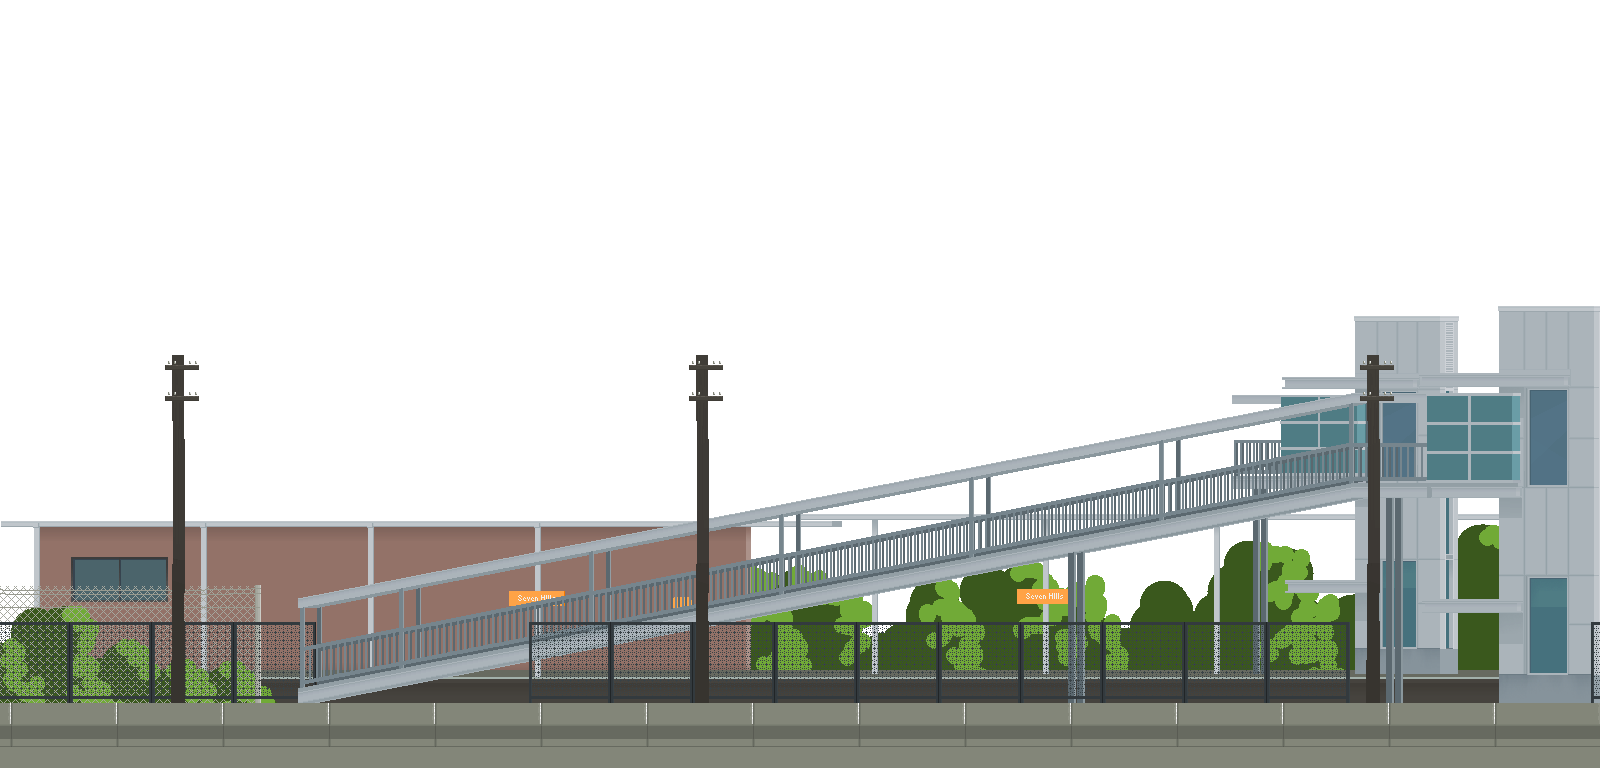
\includegraphics[scale=1.0, width=\textwidth]{latex-images/direct-daylight.png}
\end{figure}
\vfill{}
\vfill{}
\Large{Alex Tan}\\
\Large{\today}\\
\end{center}
\thispagestyle{empty}
\end{titlepage}	

\tableofcontents
\thispagestyle{empty}
\clearpage

\setcounter{page}{1}

\section{Introduction}
The Direct Daylight Project is a 2.5D, retro-style, story-driven game, with its key themes centred around nostalgia and discovery.
\subsection{The Team}
\subsubsection{Alex Tan}
\textbf{Role:} Technical Lead\\
\textbf{Google Drive:} \lstinline{torc.madra@hotmail.com}\\
\textbf{Trello:} \lstinline{@alextan60}\\
\subsubsection{Brian Huang}
\textbf{Role:} Musical Lead\\
\textbf{Google Drive:} \lstinline{brianhuang324@gmail.com}\\
\textbf{Trello:} \lstinline{}\\
\subsubsection{Dylan Kroft}
\textbf{Role:} Graphic Designer\\
\textbf{Google Drive:} \lstinline{dylankroft@gmail.com}\\
\textbf{Trello:} \lstinline{@dylankroft}\\
\subsubsection{Xing Lin}
\textbf{Role:} Artistic Lead\\
\textbf{Google Drive:} \lstinline{elevatedcross.ing@gmail.com}\\
\textbf{Trello:} \lstinline{@xinglin7}\\
\subsection{Open Positions}
\begin{enumerate}
\item \textbf{Artist}
\begin{itemize}
\item for drawing people
\end{itemize}
\item \textbf{Scriptwriter}
\begin{itemize}
\item for fleshing out and writing the dialogue of the story
\end{itemize}
\item \textbf{Voice Actors}
\begin{itemize}
\item after the script has been finalised
\item if possible
\end{itemize}
\end{enumerate}
\subsection{Weekly Meetings}
There will be weekly meetings held in-person to discuss the progress of the project. These will generally be held on Sunday afternoons. Contact Alex for more information.
\section{Documentation}
\subsection{Google Drive}
\paragraph{}
The majority of the project documentation can be found in the shared Google Drive folder. Contact Alex for more information.
\paragraph{}
The main document \textit{Direct Daylight} contains detailed information about the game including the overall themes, mechanics, gameplay, storyline, progression, and the implementation technicalities.
\paragraph{}
The \textit{Artwork} document is used for documenting details about art in the game.
\subsection{Trello}
\paragraph{}
Trello is an app used for organising and planning out tasks, which helps in tracking the progress of the project.
\begin{itemize}
\item Sign up for Trello at \url{https://trello.com}
\item Accept the Trello board invitation at \\ \url{https://trello.com/invite/b/CW6IRbz0/b1605676bf57e5327f3cd156d03979d7/direct-daylight-game}
\item The Trello Board can now be edited at \url{https://trello.com/b/CW6IRbz0}
\end{itemize}
\begin{figure}[H]
\centering
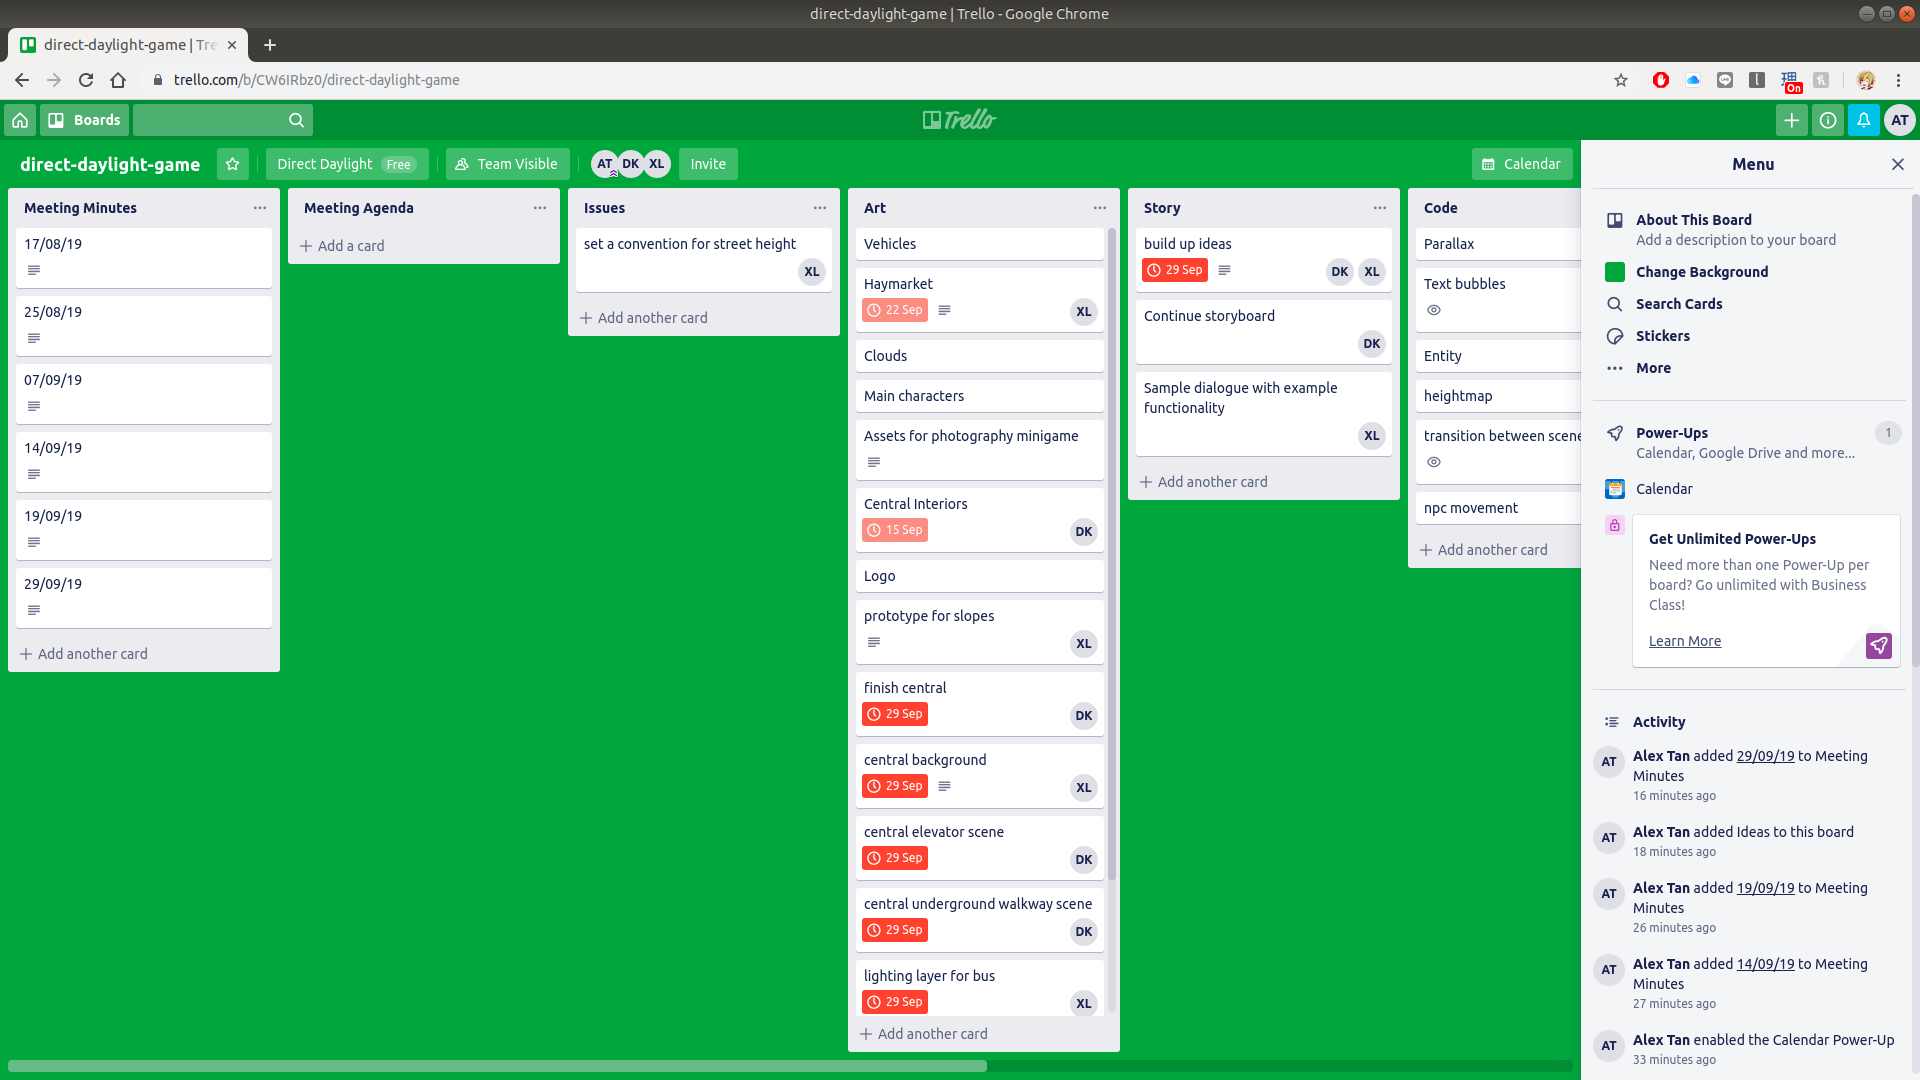
\includegraphics[scale=1.0, width=\textwidth]{latex-images/trello}
\caption{\textit{Direct Daylight} Trello Board}
\end{figure}
\paragraph{}
Please try to stick to the schedule and meet deadlines so that the project can progress swiftly. Make sure you check the Trello board before each meeting to ensure you have completed the assigned tasks.
\paragraph{}
Previous meeting minutes, as well as the agenda for the next upcoming meeting will also be on Trello.
\section{SSH \& Git}
\paragraph{}
This section covers how to download the project files, make changes, and sync these changes so that it can be viewed by the whole team.
\subsection{Generating an SSH Key}
\paragraph{}
You will first need an SSH key to gain access to the project files. Think of an SSH key as like a special password. To get started, follow the following instructions.
\begin{enumerate}
\item Open a terminal.
\item Run \lstinline{ssh-keygen}.
\begin{itemize}
\item You will be prompted for a location to save the \lstinline{id_rsa.pub} file. Leave this blank to save it in the default location.
\end{itemize}
\item Take note of where the \lstinline{id_rsa.pub} file is stored. You can find the location of the file in the command prompt.
\begin{itemize}
\item On Windows, this is usually \lstinline{C:\Users\your_username/.ssh/id_rsa.pub}
\item On Mac, this is usually \lstinline{/Users/your_username/.ssh/id_rsa.pub}
\item On Linux, this is usually \lstinline{~/.ssh/id_rsa.pub}
\end{itemize}
\item Send the \lstinline{id_rsa.pub} file to Alex.
\end{enumerate}
\paragraph{}
Note that you will also have a file named \lstinline{id_rsa} in the same directory. This is known as your private key and should \textbf{not} be shared with anyone.
\subsection{Setting Up Git}
\paragraph{}
Git is a tool for keeping track of changes in project files, and for coordinating work between multiple people across the team. You can think of it as a more sophisticated version of Google Drive, or Microsoft OneDrive.
\paragraph{}
To get started, first check if you have git installed, and download it if it is not installed.
\begin{itemize}
\item On \textbf{Windows}, open the Start Menu and search for git. Unless you have used git before, it probably will not be installed. Visit \url{https://git-scm.com/download/win} to download and install git.\\\\
To check if it installed correctly, open the Start Menu and search for git. After opening git, a command prompt should open. Now run \lstinline{git --version}.
\item On \textbf{Mac}, you may or may not have git installed. You can check by opening a terminal and running \lstinline{git --version}. If git is not installed, visit \url{https://git-scm.com/download/mac} to download and install git.\\\\
To check if it is installed correctly, open a terminal, and run \lstinline{git --version}.
\item On \textbf{Linux}, you may or may not have git installed. You can check by opening a terminal and running \lstinline{git --version}. If git is not installed, visit \url{https://git-scm.com/download/linux} and follow the instructions.\\\\
To check if it is installed correctly, open a terminal, and run \lstinline{git --version}.
\end{itemize}
\subsection{Command Prompt Basics}
\paragraph{}
There are numerous commands that can be run in the command prompt. The following are the most useful to get you started.
\begin{center}
\begin{tabular}{ll}
\lstinline!ls! & Lists all the files and directories in your current directory.\\ 
\lstinline!pwd! & Prints the location of your current directory.\\
\lstinline!cd directory_name! & Navigates to the specified directory (relative to where you currently are).\\
\lstinline!cd .. ! & Navigates to the parent directory (relative to where you currently are).\\
\end{tabular} 
\end{center}
\subsection{Cloning the Repo}
\paragraph{}
We first need to download the project files. In the git command line, navigate to somewhere you want to download the project to, and then run the following command.
\begin{lstlisting}
git clone git@directdaylight.com:direct-daylight-game
\end{lstlisting}
\paragraph{}
This will create a new folder named \lstinline{direct-daylight-game} and download the project into that folder.
\subsection{Git Primer}
\subsubsection{Committing Files}
\paragraph{}
Once you have made changes to the project files and are happy with your changes, you are ready to \textbf{commit} your changes. Firstly you will need to add the files to the commit. To add all (modified) files to the commit, navigate to the top folder in the project and run the following.
\begin{lstlisting}
git add .
\end{lstlisting}
\paragraph{}
Here the \lstinline{.} indicates that you are adding everything in the current directory.
\paragraph{}
You can also add individual files or directories.
\begin{lstlisting}
git add background2.png
\end{lstlisting}
\paragraph{}
To check that you have added the correct files, run the following command.
\begin{lstlisting}
git status
\end{lstlisting}
\paragraph{}
This displays basic information about the current state of the project, such as any changes to files you have made, and information about commits.
\paragraph{}
If you have successfully added your files to the commit, you should see a message like the following.
\begin{figure}[H]
\centering
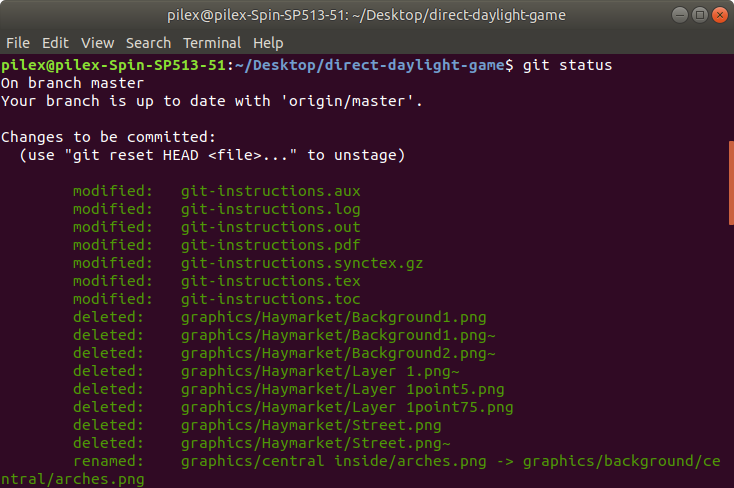
\includegraphics[scale=1.0, width=0.8\textwidth]{latex-images/git1}
\caption{}
\end{figure}
\paragraph{}
If this is your first time using \lstinline{git}, you will also need to run the following commands. Replace the email and name with your real email and name.
\begin{lstlisting}
git config --global user.email "johnsmith@gmail.com"
git config --global user.name "John Smith"
\end{lstlisting}
\paragraph{}
To commit the files you have added, you will need to provide a commit message, which is a short but descriptive message for describing what you have changed in this commit e.g. \lstinline{"added animation"}.
\begin{lstlisting}
git commit -m "added animation"
\end{lstlisting}
\paragraph{}
After you have committed your changes try running \lstinline{git status} again, and you should see a message like the following.

\subsubsection{Pushing Your Own Changes}
\paragraph{}
You have now committed your changes to the project, however your changes are not yet visible to the whole team. At this point, you can make more changes and make more commits if you would like. Once you are ready, you can share the changes with the whole team by running the following command.
\begin{lstlisting}
git push origin master
\end{lstlisting}
\paragraph{}
This pushes your commits to the main server. Think of it as uploading your changes.
\paragraph{}
Under certain situations, you may not be able to push to the server. To solve this, read the following sections.
\subsubsection{Pulling Other People's Changes}
Other people may be working on the project as well, and will be committing and pushing changes using \lstinline{git commit} and \lstinline{git push origin master} the same way that you have been doing. Git does \textbf{not} automatically download these changes. To retrieve the latest version of the project, run the following command.
\begin{lstlisting}
git pull origin master
\end{lstlisting}
\paragraph{}
This may fail if you have edited files but not yet committed them. This is because these changes may potentially be overwritten. The simplest way to solve this is to commit your changes. Alternatively, you can \textbf{stash} your changes. We will discuss stashing later on.
\paragraph{}
If you are having trouble pushing to the server, it may be because someone else has already made changes using \lstinline{git push origin master}, and you are still on the old version of the project. In this case, running \lstinline{git pull origin master}, and then pushing your changes as usual using \lstinline{git push origin master} should fix the issue.
\paragraph{}
However, if someone else has changed a file that you have worked on, or has deleted a file that you have worked on, \lstinline{git pull origin master} will fail. In this case you will get a \textbf{merge conflict}. We will discuss how to solve merge conflicts in the next section.
\subsubsection{Merge Conflicts}
\paragraph{}
A \textbf{merge conflict} typically occurs when two people have changed the same lines in a file, or if one person has deleted a file whilst somebody else was modifying it.
\paragraph{}
More info: \url{https://www.atlassian.com/git/tutorials/using-branches/merge-conflicts}
\subsubsection{Stashing}
\paragraph{}
Stashing temporarily shelves (or \textit{stashes}) changes you've made, so that you can work on something else, and come back and re-apply those changes. This is useful if you are working on something, but you aren't quite ready to commit and want to work on something else.
\paragraph{}
More info: \url{https://www.atlassian.com/git/tutorials/saving-changes/git-stash}
\subsubsection{Viewing the Project History}
\paragraph{}
You can view the history of the project using the following command.
\begin{lstlisting}
git log
\end{lstlisting}
\paragraph{}
This lists out all the commits so far including the commit author and commit message of each commit.
\section{Code}
\paragraph{}
The game code is written in Java, using the Processing graphics library. You can find some introductory resources at \url{http://directdaylight.com/learn-processing/learn-processing-presentation.pdf} as well as the official documentation at \url{https://processing.org/reference/} to help get you started.
\subsection{Eclipse}
\paragraph{}
To edit the code and run the game, it is recommended that you use an Integrated Development Environment (IDE) such as Eclipse. The following section will go through setting up Eclipse.
\subsubsection{Setting Up Eclipse}
\begin{enumerate}
\item You will first need to download Eclipse from \url{https://www.eclipse.org/downloads/} and install it. Inside the installer, make sure you choose the Java edition.
\item When you first run Eclipse, you will get a prompt asking for a working directory. You can pick any folder you want, or just use the default.
\item Once Eclipse has loaded, you will be greeted with the Welcome Page. Click on the \textit{Workbench} button in the top right.
\item Now in the \textit{Package Explorer} tab on the left, right-click and select \textit{Import}.
\item Select \textit{General}, then \textit{Existing Projects Into Workspace} and click \textit{Next}.
\item Select \textit{Root Directory}, then click on \textit{Browse}. Navigate to where you have saved the \lstinline{direct-daylight-game} folder. Make sure that under the \textit{Projects} tab, \lstinline{direct-daylight-game} is selected. Also make sure that under the \textit{Options} tab, the \textit{Copy Projects Into Workspace} checkbox is \textbf{not} checked. 
\item Finally, click \textit{Finish}.
\end{enumerate}
\subsubsection{Running the Game}
\paragraph{}
The \lstinline{main} function is located under \lstinline{main/Game.java}. 
\paragraph{}
In Eclipse, navigate to \lstinline{direct-daylight-game/src/main/Game.java}, then click on the green run button located on the top toolbar. This will run the game!
\end{document}